\chapter{Knowledge Graph Visualization Tool}
\label{chap:OWLViz}
Many existing knowledge graph visualizations are restricted to displaying certain types of relationships. 
Most commonly, a class hierarchy of an ontology is visualized for the user. Other graph visualization tools have built in features capable of 
displaying relationships between instantiated classes or \textit{NamedIndividuals}.
A few of these graph visualizers are mentioned in \nameref{chap:Related_work}.

What we didn't find is a graph visualizer capable of displaying complex class expressions, therefore, we decided to develop our own graph visualizer, 
which is capable of displaying class hierarchies with complex constructs.

This chapter will present the main features of our \textit{Knowledge Graph Visualization Tool}, where explain explain its capabilities and limitations.

\section{Main concept}
\label{sec:MainConceps}

We present you our three main concepts, which are incldued in the \textit{Knowledge Graph Visualization Tool}:
\begin{itemize}
    \item \textbf{Visualization of Class Hierarchy}: Our primary goal is to visualise a class hierarchy, where class relations are visible to the 
    user and visualise complex class expressions as a part of the corresponding class. This will be done as compact as possible. 
    Furthermore to differentiate between classes and class expressions we aim to make such distinction via different coloring. 
    Additionally, we aim to keep the amount of nodes and edges low, to reduce clutter in the graph, making exploring graph easier and 
    increase performance of visualizing such graphs.  
    \item \textbf{Query Builder}: To clarify the relations between the queries, we implement a query builder that, given a class, can point to other classes through the relation, 
    which in turn can point to further classes through another relation, as long as the user desires or there are no further relations. 
    No \textit{SPARQL} knowledge is required query language, making it usable for the user. 
    The \textit{Query Builder} outputs a filtered graph with the selected triples and generates a \textit{SPARQL} query.
    \item \textbf{Rule Based Inference}: Our thesis relies on running inference over \textit{mixing} 
    we implement an inference tool running reasoning over our ontology, to find motions, analogously to \nameref{subsection:MixingActionSWRL}.
    The result is visualized in a graph and a sequence of actions in natural language are generated, to highlight inferred knowledge.  
\end{itemize}

\section{Features}

\begin{figure}[H]
    \centering
    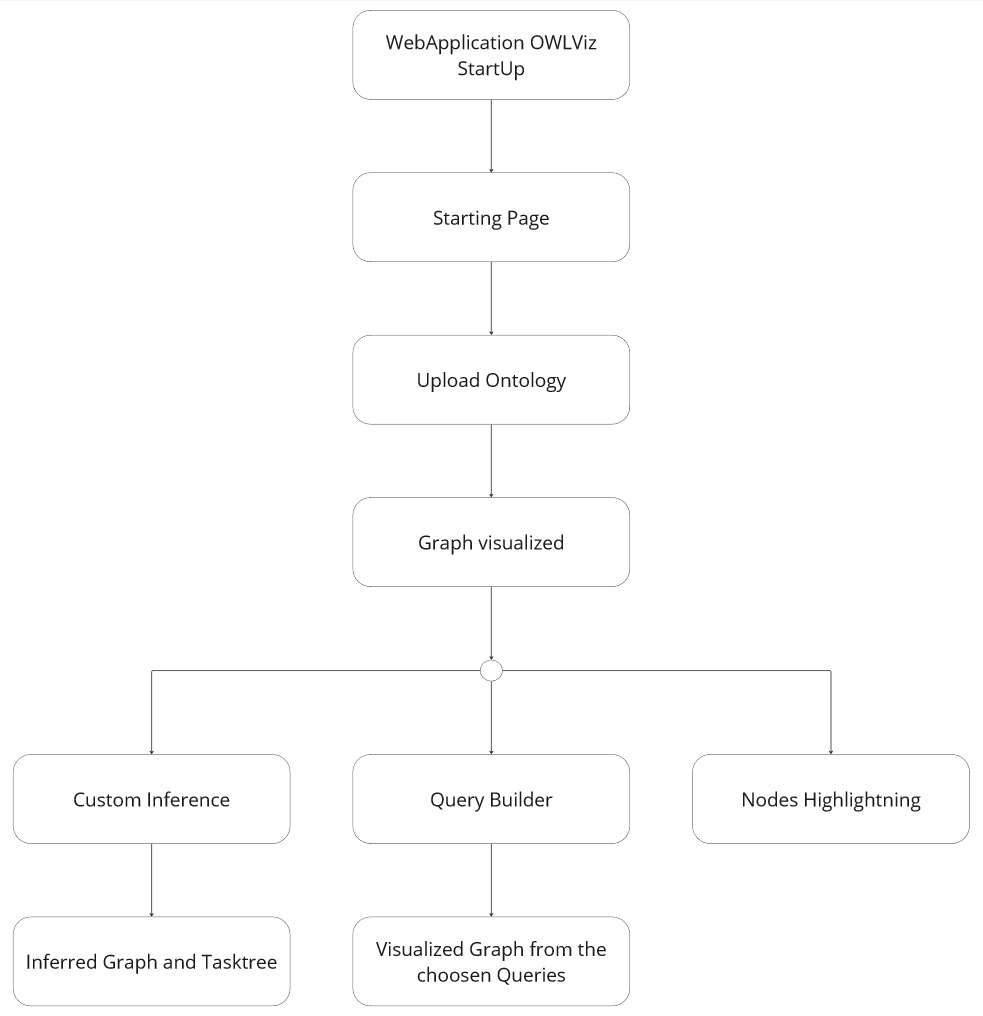
\includegraphics[scale=0.35]{Graphics/architecture_simplified.jpg}
    \label{fig:OWLViz_architecture}
    \caption{Architecture chart for the \textit{Knowledge Graph Visualization Tool} framework}
\end{figure}

\subsection{Graph Visualization}
In this section, we present a simple example of our framework, from processing the ontology to visualization in the web application. 
For this purpose, we create a small and simple ontology to explain the basic visualization of an ontolgy. 
The visualization library \textit{vis.js} \cite{visjs} has been used to create graph visualization in web-browsers.

\begin{figure}[H]
    \centering
    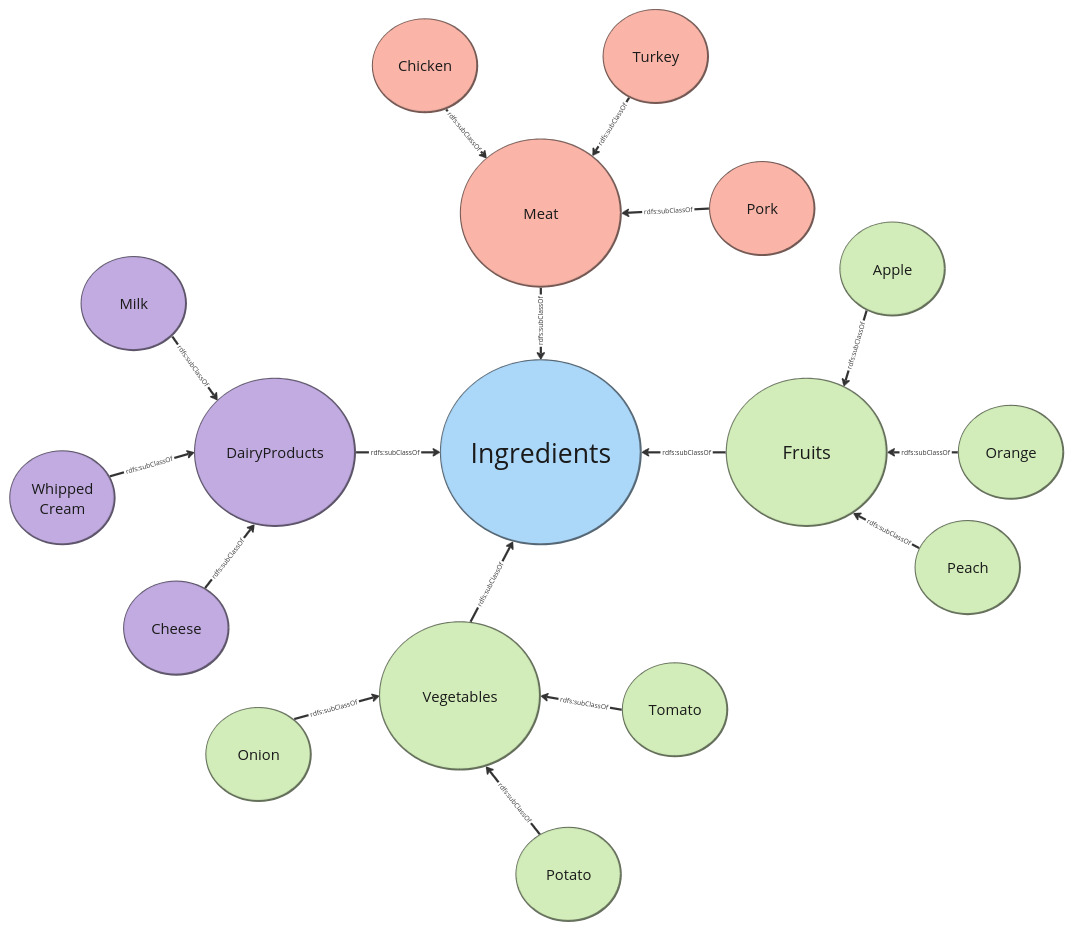
\includegraphics[scale=0.4]{Graphics/simple_ontology.jpg}
    \caption{Trivial example of an ontology}
\end{figure}
    
The ontology created for this purpose aims to provide a simple representation of various food products. 
It includes superclass categories such as \textit{Fruits, Vegetables, Meat, and Dairy Products}, as well as subclasses like \textit{Apple} and \textit{Orange}, 
which are subclasses of the \textit{Fruits} superclass. 
This visualization is a simple visualization of a class hierarchy of food products, where each node is connected via 
a directed edge labeled with \textit{subClassOf}.

\subsection{Graph Processing}
The core component of the graph visualizer is the visualization of a hierarchy of classes. In this hierarchy, two nodes are connected by a directed edge, 
where the source node is the child node and the target node is the parent node. All edges are labeled either as \textit{subClassOf} or \textit{equivalentClass}.

To create the visualization from the graph, the ontology is parsed, and a triple matching process is applied to identify 
all classes that use \textit{subClassOf} or \textit{equivalentClass} as predicates.

By default, all nodes are uniformly colored green. However, in the \textit{mixing} and \textit{FoodCutting} \cite{Kuempel2024} ontologies, 
additional colors are used to highlight differences.
\begin{figure}[H]
    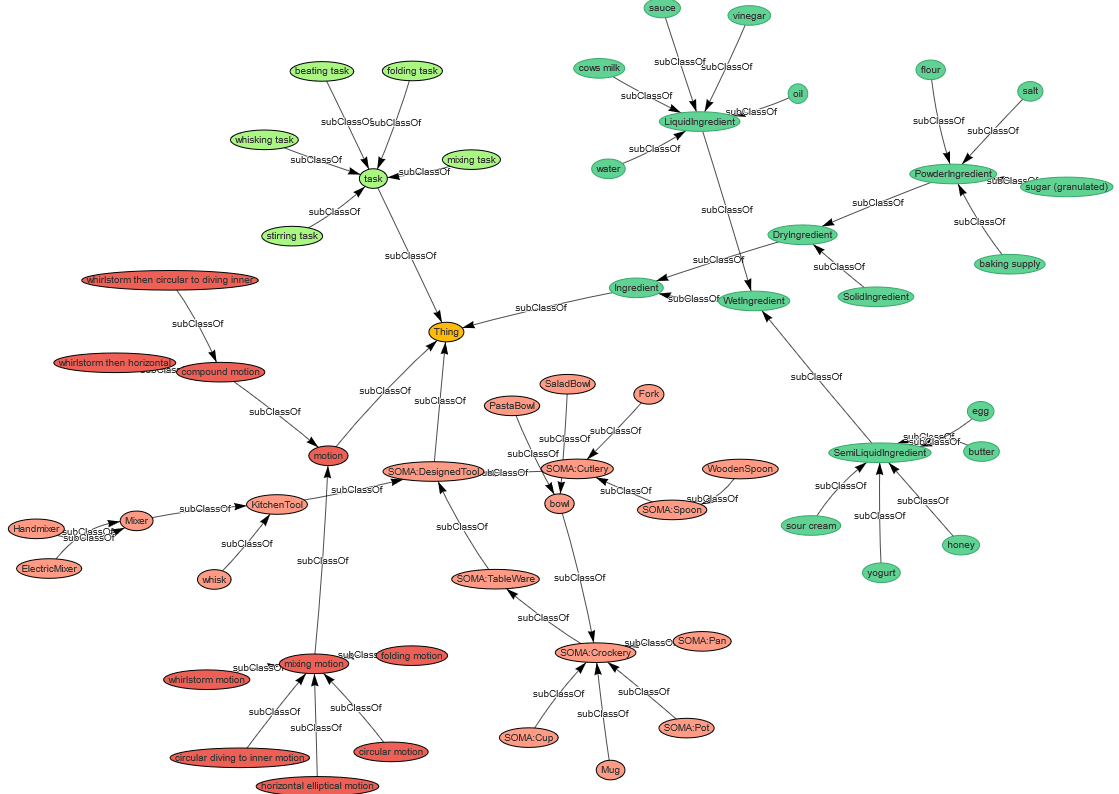
\includegraphics[scale=0.5]{Graphics/OwlVisualizer/graphProcessing1.png}
    \centering
    \caption{Processed Class Hierarchy}
\end{figure}

The graph visualizer is also capable of visualizing complex class expressions. 
However, it is essential to understand why the parsed expressions should not be used directly, as illustrated in figure \ref{fig:graphProcessing2}. 
Blank nodes and meta information associated with these expressions are generally useless to the user. 
This type of visualization is not compact, and users unfamiliar with ontology parsing will find it confusing and uninformative. 
Additionally, visualizing each parsed node increases the number of nodes and edges, which decreases performance of creating the graph visualization. 
Therefore, a more compact visualization of complex restrictions is necessary to ensure clarity and maintain optimal performance.

\begin{figure}[H]
    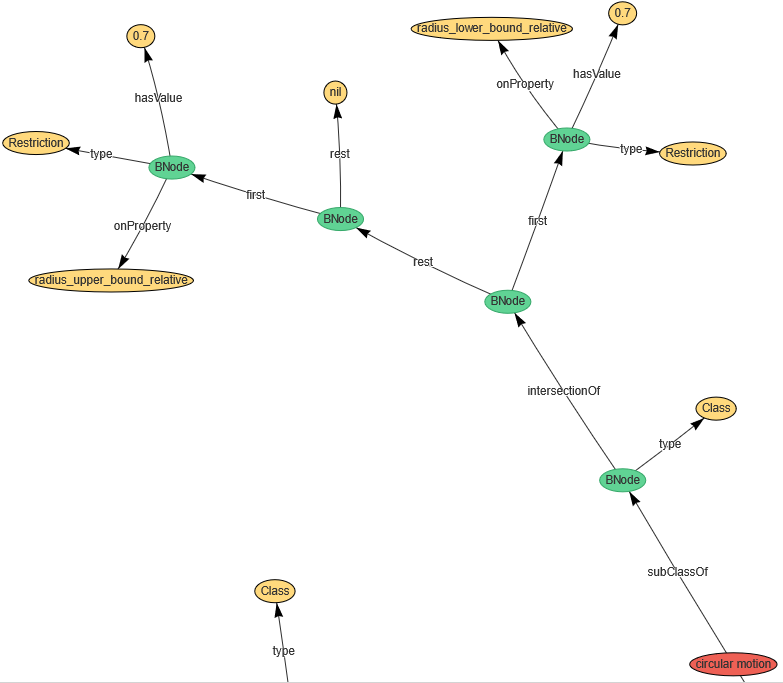
\includegraphics[scale=0.5]{Graphics/OwlVisualizer/graphProcessing2.png}
    \centering
    \caption{Visualize parsed class restrictions}
    \label{fig:graphProcessing2}
\end{figure}

To achieve a compact representation of class expressions, we recursively traverse the parsed class expression, 
searching for essential information such as the relations used and their corresponding values. 
All blank nodes are implicitly skipped and not visualized. Additionally, meta information are excluded.

The visualizer can also handle nested expressions, as well as intersections and unions. Each \textbf{AND} node indicates that all connected elements belong to the intersection.
Similarly, each \textbf{OR} node indicates that all connected elements belong to the union.

In the figure \ref{fig:graphProcessing3}, the following expression is visualized:

CircularMotion \textit{subClassOf} (radius upper bound relative value 0.7) and (radius lower bound relative value 0.7)

\begin{figure}[H]
    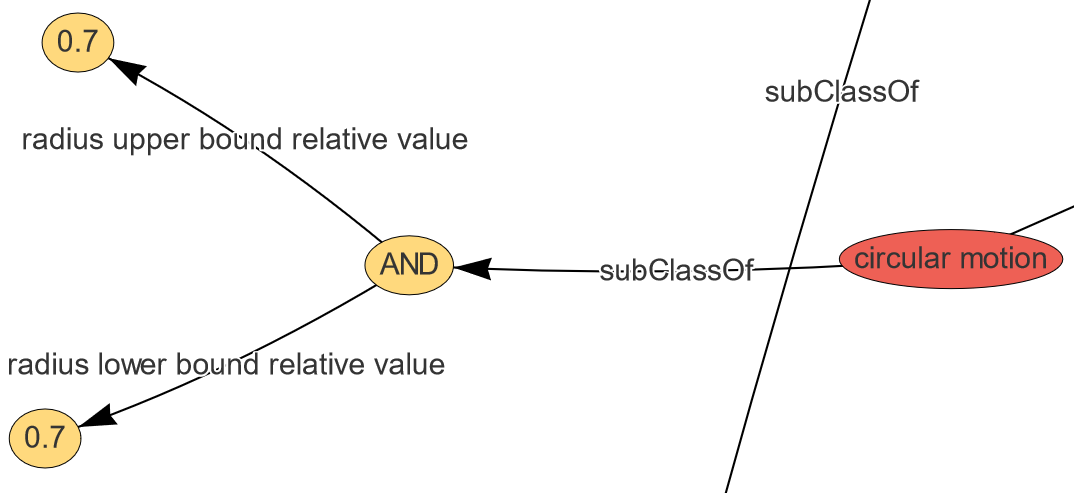
\includegraphics[scale=0.3]{Graphics/OwlVisualizer/graphProcessing3.png}
    \centering
    \caption{Compact representation of class expression}
    \label{fig:graphProcessing3}
\end{figure}

\subsection{Load Ontology}

By pressing the \textit{Load Ontology} button, users can load a wide range of ontologies that have the \textit{.owl} file extension.
Upon selecting the ontology, the \textit{Knowledge Graph Visualization Tool} begins parsing the ontology to process the ontology. 
Once the processing is complete, a visual representation of the ontology is created, which can be explored by the users freely. 


\begin{figure}[H]
    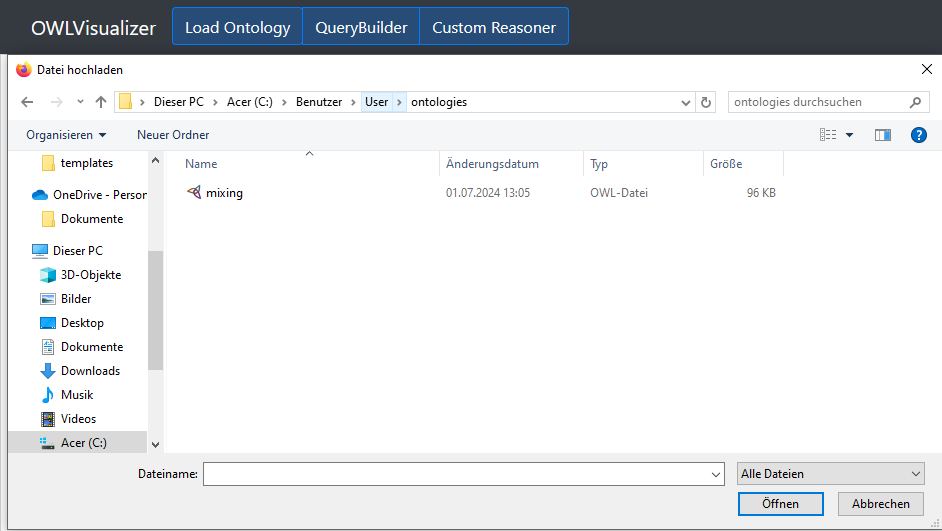
\includegraphics[scale=0.35]{Graphics/OwlVisualizer/loadOntology1.png}
    \centering
    \caption{Loading Ontology}
    \label{fig:loadOntology1}
\end{figure}

Attempting to load any other file types results in an error message being displayed on the website. 
When a user tries to upload a file that does not have the \textit{.owl} extension, the \textit{Knowledge Graph Visualization Tool} notifies 
the user that the file extension is not supported by this tool, via an error message. 

\begin{figure}[H]
    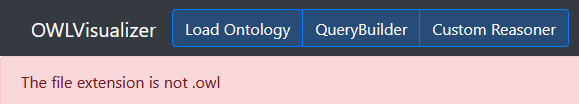
\includegraphics[scale=0.5]{Graphics/OwlVisualizer/loadOntology2.png}
    \centering
    \caption{\textbf{Error}: Unsupported File Type}
    \label{fig:loadOntology2}
\end{figure}

Additionally, if an ontology can't be parsed, an error message is thrown that ontology couldn't be
loaded properly. Whenever this issue is encountered during the parsing of the selected ontology, it immediately stops and triggers an error notification. 
This message informs the user that there was a problem with loading the ontology, possibly due to a formatting error or an unsupported structure within the file. 
This error message informs the user of this particular issue; the \textit{Knowledge Graph Visualization Tool} doesn't attempt to deal with this problem.

\begin{figure}[H]
    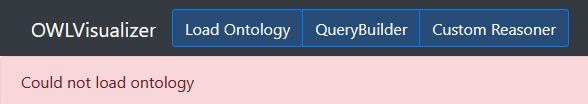
\includegraphics[scale=0.5]{Graphics/OwlVisualizer/loadOntology3.png}
    \centering
    \caption{\textbf{Error}: Ontology Load Failure}
    \label{fig:loadOntology3}
\end{figure}

\subsection{Search Classes}
The \textit{Knowledge Graph Visualization Tool} includes a feature that suggests classes, which are visualized as nodes, 
for users to focus on, improving their ability to navigate and understand complex networks.

\begin{figure}[H]
    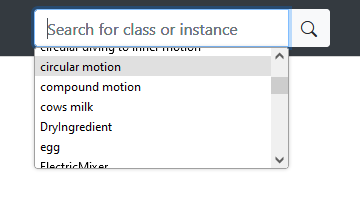
\includegraphics[scale=0.6]{Graphics/OwlVisualizer/searchClass1.png}
    \centering
    \caption{Search bar suggesting available classes}
\end{figure}

The key implementation for this feature is a search bar that suggests all visualized classes. 
Any nodes belonging to a class restriction are not suggested. 
The available suggestions are sorted in descending order, allowing users to easily search
for classes and explore the class hierarchy without assuming prior familiarity with the ontology.

\begin{figure}[H]
    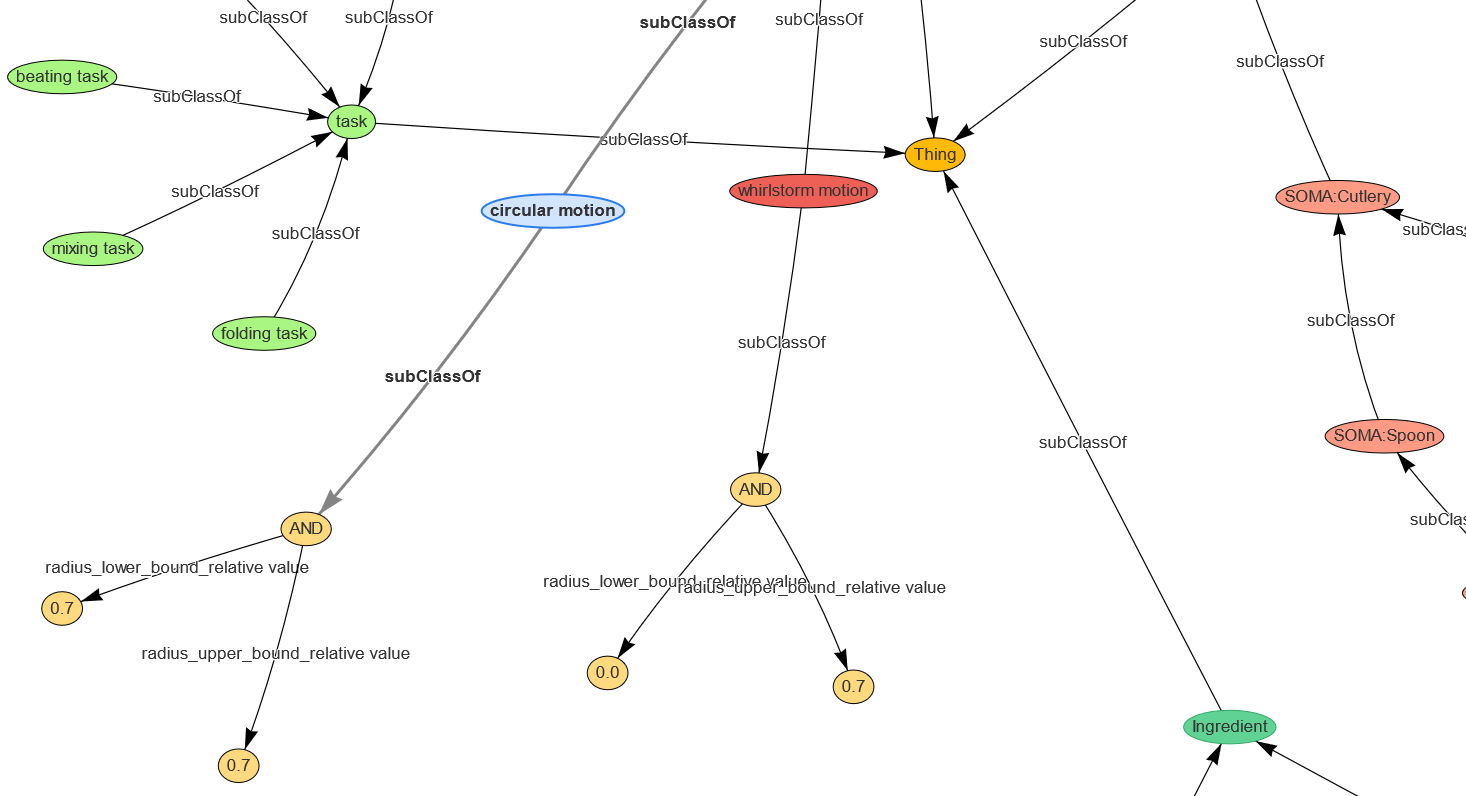
\includegraphics[scale=0.25]{Graphics/OwlVisualizer/searchClass2.png}
    \centering
    \caption{Focus node}
\end{figure}

Users can press \textbf{Enter} inside the search bar or click the search button to immediately focus on the chosen class. 
Focusing on the class is achieved by zooming to the respective node and highlighting it. 
This allows users to quickly identify the corresponding node along with all of its parent and child nodes.

\subsection{Custom Inference - Mixing}
To understand which motion can be inferred using the \textit{mixing} ontology, we created
the \textit{Custom Inference} (see \nameref{chap:Data_representation}) feature. The user simply selects the task to 
execute and the ingredients to include in the specific task. 
\begin{figure}[H]
    \centering
    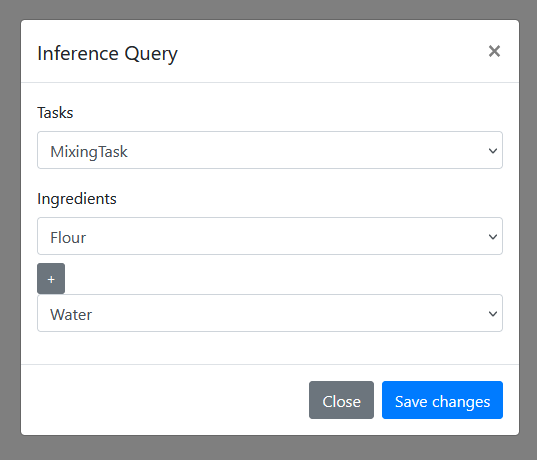
\includegraphics[scale=0.45]{Graphics/inference_user_input.png}
    \caption{Select Task and Ingredients.}
\end{figure}
The \textit{Custom Inference} feature generates a graph that contains assertional knowledge, such as the task and the ingredients. 
Furthermore, the inferred motion along with its parameters is visualized for the user in a single graph. 
Additionally, a sequence of steps is generated, which the robot can execute to successfully complete its task. 
To achieve this, the form data is processed, and a reasoning process is initiated to run inference over our \textit{SWRL} rules, extract all inferred knowledge, 
and create a visualization and a sequence of actions.

\begin{figure}[H]
    \centering
    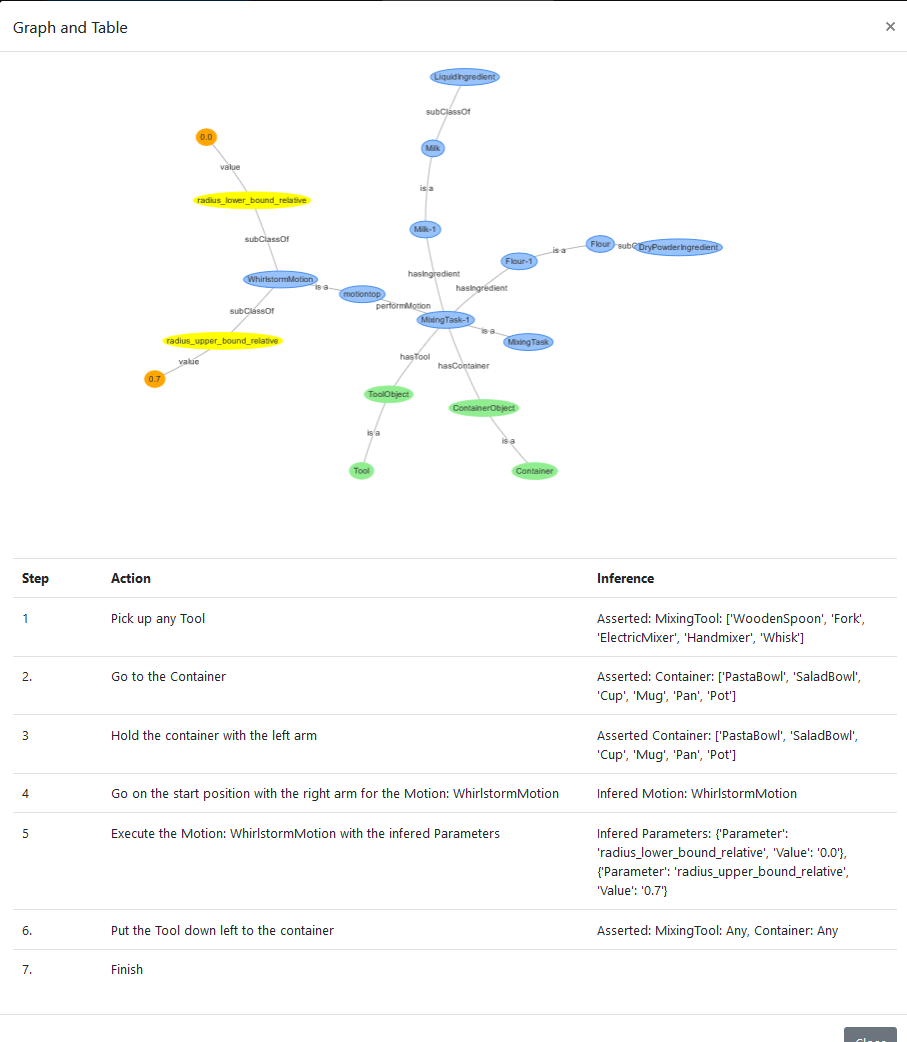
\includegraphics[scale=0.5]{Graphics/new_inference_graph.png}
    \caption{Visualize Graph and Sequence of Actions.}
    \label{fig:graph_inferred}
\end{figure}
\subsection{Query Builder}
The \textit{Query Builder} is a feature that provides users with suggested triples, allowing them to explore the graph in an intuitive manner.
No \textit{SPARQL} knowledge is required. This feature generates a visualization of the selected triples and constructs a \textit{SPARQL} query, 
which can be modified to the users needs.

\paragraph{Triple Matching}
Triple Matching allows users to select a subject, predicate, and object to explore the graph. 
At the beginning of the triple matching process, all classes are available as subjects. 

\begin{figure}[H]
    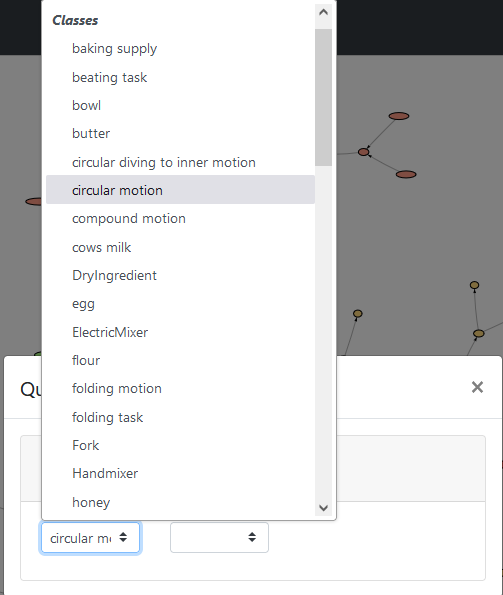
\includegraphics[scale=0.4]{Graphics/OwlVisualizer/queryBuilder1.png}
    \centering
    \caption{View Possible Subjects for Selection}
\end{figure}

Only predicates that appear as edge labels connected to the subject in the graph are suggested. 

\begin{figure}[H]
    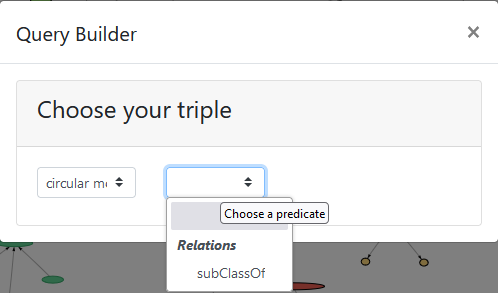
\includegraphics[scale=0.4]{Graphics/OwlVisualizer/queryBuilder2.png}
    \centering
    \caption{View Possible Predicates for Selection}
\end{figure}
Similarly, only objects connected to the subject via the selected edge are proposed. 

\begin{figure}[H]
    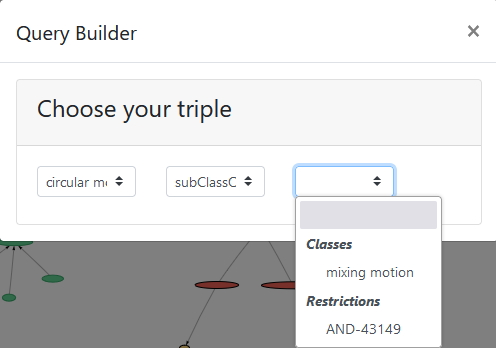
\includegraphics[scale=0.4]{Graphics/OwlVisualizer/queryBuilder3.png}
    \centering
    \caption{View Possible Objects for Selection}
\end{figure}
Once a triple is selected, the user can continue to explore the graph based on the previously chosen triples.

All complex class expressions are processed in a single triple matching step, whereas navigating through the class hierarchy occurs incrementally.

Whenever a triple is selected, the \textit{Query Builder} creates a tab with two items, one item visualizes the graph, the other item 
contains a \textit{SPARQL} query. 

\paragraph{View Graph}
In the \textit{View Graph}, users can inspect the graph based on their selection of triples. 
This view is a subgraph, which makes it easier to inspect the relationships between classes and classes with complex class expressions. 
Each class expression is displayed in a separate view, allowing users to focus on each class expression independently, which also reduces clutter in the graph. 
The class hierarchy has its own view, which can be incrementally updated with new classes to view hierarchical relationships. 
Separating the views ensures that users can navigate and explore different aspects of the graph, while also improving their comprehension of the ontology.

\begin{figure}[H]
    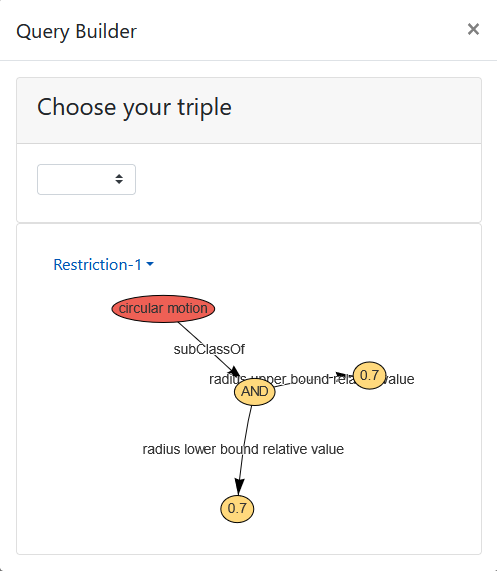
\includegraphics[scale=0.5]{Graphics/OwlVisualizer/queryBuilder4.png}
    \centering
    \caption{Graph View}
\end{figure}

\paragraph{SPARQL Query}
A \textit{SPARQL ASK} query is generated for each chosen triple. If the triple is querying the hierarchy, the \textit{SPARQL} query for querying the hierarchy is updated with the newest triples.
For each complex class expression, a separate query corresponds to the view of the subgraph.

This query is a queryable triple pattern that asks if this query pattern has a solution or not. 
Users can then independently modify and adapt this pattern to suit their specific needs. 
This feature will help users unfamiliar with querying ontologies by providing them with the triple pattern.
\begin{figure}[H]
    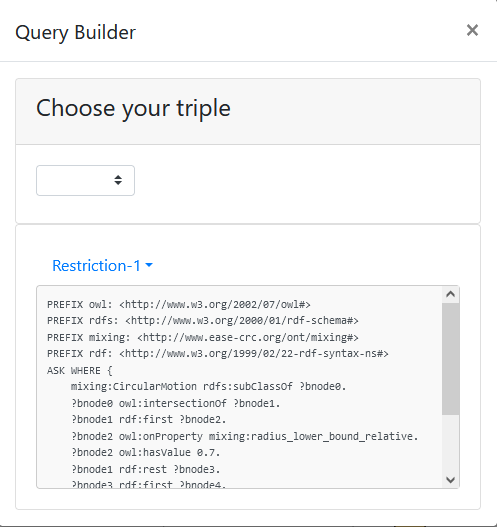
\includegraphics[width=0.5\textwidth]{Graphics/OwlVisualizer/queryBuilder5.png}
    \centering
    \caption{\textit{SPARQL} View}
\end{figure}

\section{Limiations}

\paragraph{Using vis.js and Visualization of NamedIndividuals}

The graph visualization library \textit{vis.js} suffers from poor performance when handling large graphs, acknowledged by its developers \cite{visjs}. 
This limitation primarily stems from the physics simulation used in its force-directed graph layout, 
which attempts to arrange nodes by separating and clustering them based on their connections. 
As the number of interconnected nodes and edges grows, this process becomes increasingly time-consuming, leading to decreased performance. 
While capable of displaying relationships and attributes of instance data effectively, 
\textit{vis.js} is not optimized for handling large ontologies with numerous instantiated classes. 
Due to these limitations, functionality for visualizing such ontologies has not been implemented.

\paragraph{Inference and Reasoning}

Although we have developed a custom reasoner tailored specifically for the \textit{mixing} ontology, 
the current implementation does not support reasoning over other ontologies apart from \textit{mixing}. 
This decision was made due to runtime concerns, particularly regarding the computational complexity of \textit{SWRL} rules. 
Loading an ABox ontology, characterized by numerous NamedIndividuals and a complex class hierarchy, into this framework could severely impact performance.
Such intensive computations could potentially disrupt the usability of other features within the \textit{Knowledge Graph Visualization Tool}.